\documentclass[10pt]{article}
\usepackage[utf8]{inputenc}
\usepackage[a4paper, total={12cm, 22cm}]{geometry} % MARGIN 15.5 instead of 14 was initial

\usepackage{comment} 
\usepackage{multirow}
\usepackage[table,xcdraw]{xcolor}
\usepackage{hyperref}
\usepackage{float}
\usepackage{graphicx}
% \usepackage[dvipsnames]{xcolor}

% checkmark list
\usepackage{enumitem,amssymb}
\newlist{todolist}{itemize}{2}
\setlist[todolist]{label=$\square$}
\usepackage{pifont}
\newcommand{\cmark}{\ding{51}}%
\newcommand{\xmark}{\ding{55}}%
\newcommand{\done}{\rlap{$\square$}{\raisebox{2pt}{\large\hspace{1pt}\cmark}}%
\hspace{-2.5pt}}
\newcommand{\wontfix}{\rlap{$\square$}{\large\hspace{1pt}\xmark}}

\setlength\parindent{0pt}
\setlength{\parskip}{2em}

\usepackage{amsmath}
\usepackage{listings}
\usepackage{comment}
\usepackage{longtable}
\usepackage{markdown}
\usepackage{pdfpages}

\usepackage{biblatex}
\addbibresource{bibliography.bib}


% FOOTER AND HEADER %
\usepackage{etoolbox}
\usepackage{fancyhdr}
\pagestyle{fancy} 
\newcommand{\frontmatter}{\clearpage \cfoot{\thepage\ }
\fancyhead{}
\renewcommand{\headrulewidth}{0pt}
\setcounter{page}{1}
\pagenumbering{Roman}}
\newcommand{\mainmatter}{\clearpage \cfoot{\thepage\ of \pageref{LastPage}}
\fancyhead[LE,RO]{Group 2}\fancyhead[RE,LO]{\leftmark}
\renewcommand{\headrulewidth}{0.4pt}
\setcounter{page}{1}
\pagenumbering{arabic}}
\newcommand{\backmatter}{\clearpage \cfoot{\thepage\ }
\fancyhead{}
\renewcommand{\headrulewidth}{0pt}
\setcounter{page}{1}
\pagenumbering{alph}}
\patchcmd{\chapter}{\thispagestyle{plain}}{\thispagestyle{fancy}}{}{}
% Front page background %
\usepackage[
firstpage=true,
opacity=0.20,
angle=0,
]{background}
\backgroundsetup{contents={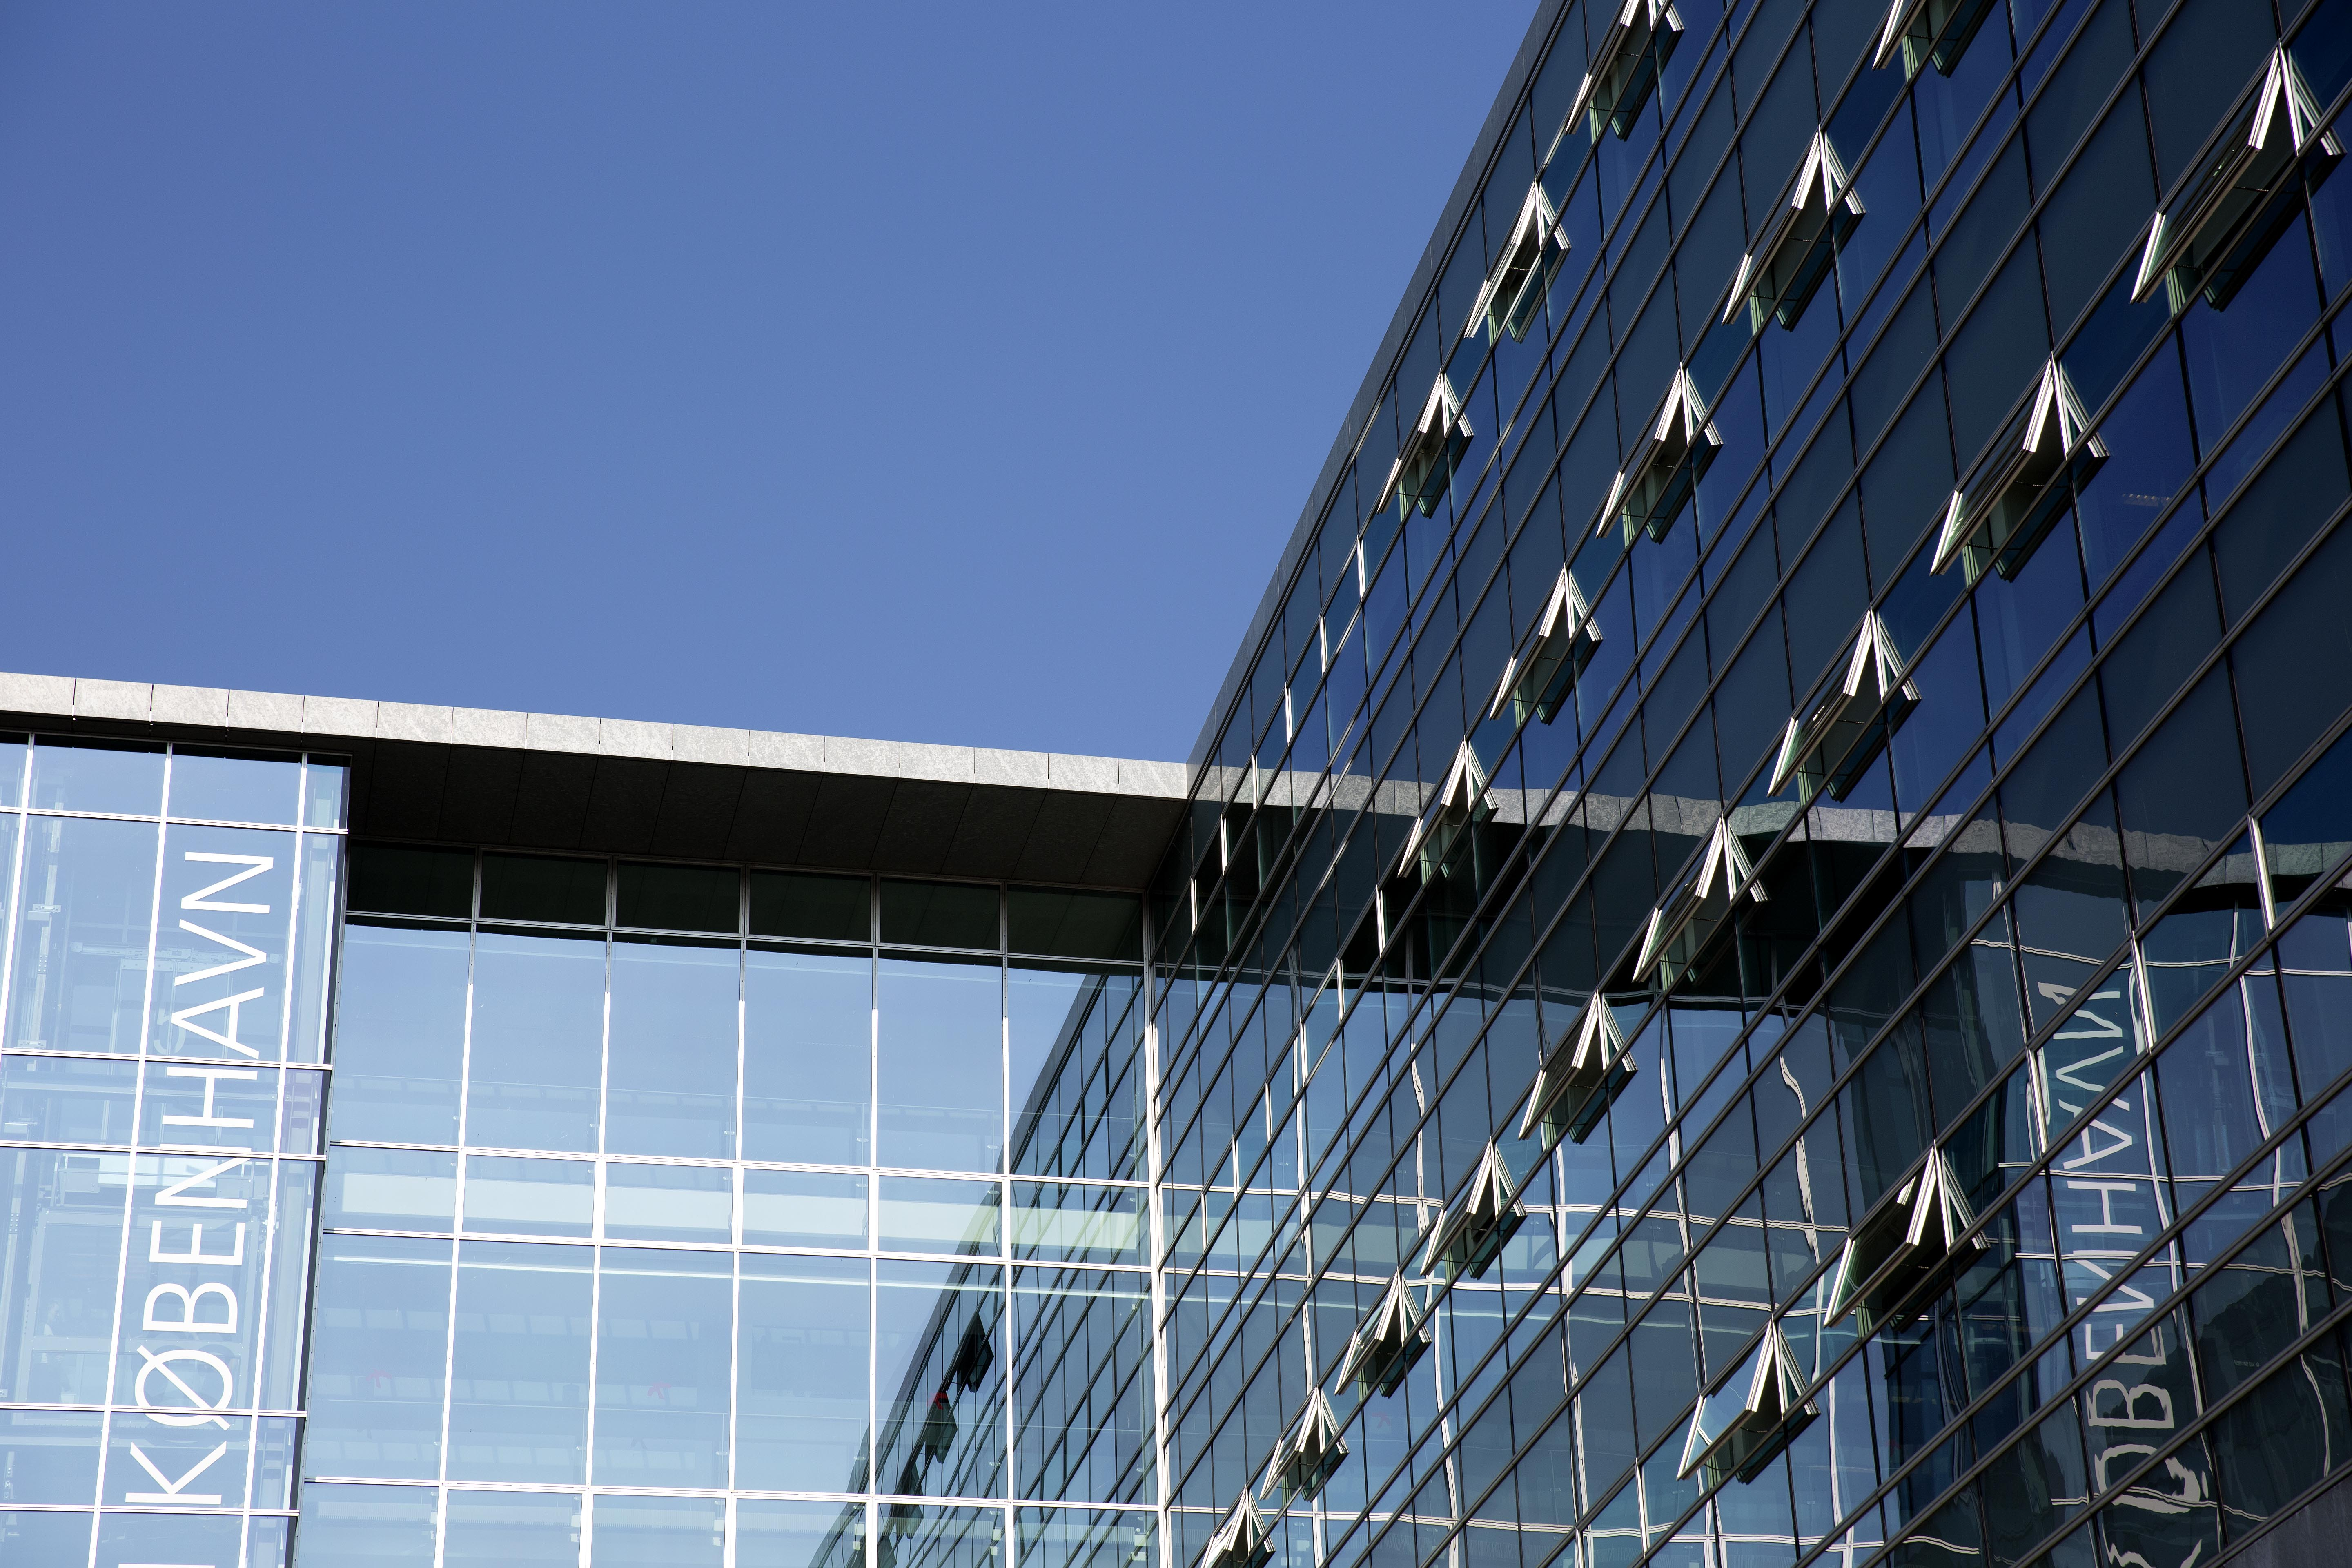
\includegraphics[scale=0.1]{template/background.jpg}}}



\begin{document}

\begin{titlepage}
    \begin{center}
        \vspace*{1cm}

        \Huge
        \textbf{Software Architecture}
        
        \vspace{0.5cm}
        
        \Large
        Delivery 1
            
        \vspace{1.5cm}
         
        \textbf{Benjamin Lindgren Christensen (belc@itu.dk)}\\
        \textbf{Christian Skovsgaard Rieck (crie@itu.dk)}\\
        \textbf{Christian Hedegaard Pliess Larsen (hecl@itu.dk)}\\
        \textbf{Gianmarco Murru (gimu@itu.dk)}\\
        \textbf{Melissa Høegh Marcher (mhom@itu.dk)}\\
            
        \vspace{1.5cm}
        
       
            
        \vfill
            
      Software Architecture, MSc\\
         KSSOARC2KU
            
        \vspace{0.8cm}
            
        
\includegraphics[width=0.5\textwidth]{template/ITU_logo_UK jpg.jpg}
            
        \Large
        Department of Computer Science\\
        Denmark\\
        Spring 2022
            
    \end{center}
\end{titlepage}

\frontmatter
\tableofcontents

\mainmatter

\section{System description}
% Describe your system briefly including its main functionality (bulleted list). In particular, you must produce one of the discussed context diagrams: the informal and formal notation. (cf. the lecture 1).

The system is a gathered overview of personal financial assets, collected from integrations to financial institutions such as banks and investment platforms. 

\subsection{Context diagram}
Figure \ref{fig:context_diagram} shows an informal context diagram of cNance, a personal finance overview system. 

\begin{figure}
  \centering
  
\includegraphics[width=0.7\textwidth]{figures/context-diagram2.png}
  \caption{Informal context diagram}
  \label{fig:context_diagram}
\end{figure}


\subsection{Overall functionality}

The system should give an overview of a citizen's financial status, which includes:
    \begin{itemize}
        \item Bank integration to show transactions
        \item Tinglysning integration to show assets like cars and houses
        \item Integration with investment platform, stocks, crypto valuta ect.
        \item SKAT integration with overview and legal assistance
        \item Graphs that show personal historical financial data and projected future financial data
        \item Data can optionally be sent to the integrations, in order for the user to receive:
        \begin{itemize}
            \item personalized bank offers
            \item notifications
        \end{itemize} 
    \end{itemize}
 

\section{Architectural analysis}
% Describe architecturally significant requirements (ASRs). The ASRs should be in the form of Quality Attribute Scenarios and these should be the output of a Quality Attribute Workshop (QAW). You should also report on the outcomes of the QAW. There should be atleast 3 scenario's for each significant architectural driver.

\includepdf[pages=-,scale=.8]{figures/slidesA4R.pdf}

\subsection{Quality Attribute Workshop}

\subsection{Quality Attribute Scenarios}


\begin{table}[h!]
\begin{tabular}{|
>{\columncolor[HTML]{F8F9FA}}l 
>{\columncolor[HTML]{F8F9FA}}l |
>{\columncolor[HTML]{F8F9FA}}l |}
\hline
\multicolumn{2}{|l|}{\cellcolor[HTML]{F8F9FA}{\color[HTML]{333333} Scenario(s):}}                                                                & {\color[HTML]{333333} } \\ \hline
\multicolumn{2}{|l|}{\cellcolor[HTML]{F8F9FA}{\color[HTML]{333333} Relevant quality attributes:}}                                                & {\color[HTML]{333333} } \\ \hline
\multicolumn{1}{|l|}{\cellcolor[HTML]{F8F9FA}{\color[HTML]{333333} }}                                 & {\color[HTML]{333333} Source: test}           & {\color[HTML]{333333} } \\ \cline{2-3} 
\multicolumn{1}{|l|}{\cellcolor[HTML]{F8F9FA}{\color[HTML]{333333} }}                                 & {\color[HTML]{333333} Stimulus:}         & {\color[HTML]{333333} } \\ \cline{2-3} 
\multicolumn{1}{|l|}{\cellcolor[HTML]{F8F9FA}{\color[HTML]{333333} }}                                 & {\color[HTML]{333333} Artifact:}         & {\color[HTML]{333333} } \\ \cline{2-3} 
\multicolumn{1}{|l|}{\cellcolor[HTML]{F8F9FA}{\color[HTML]{333333} }}                                 & {\color[HTML]{333333} Environment:}      & {\color[HTML]{333333} } \\ \cline{2-3} 
\multicolumn{1}{|l|}{\cellcolor[HTML]{F8F9FA}{\color[HTML]{333333} }}                                 & {\color[HTML]{333333} Response:}         & {\color[HTML]{333333} } \\ \cline{2-3} 
\multicolumn{1}{|l|}{\multirow{-6}{*}{\cellcolor[HTML]{F8F9FA}{\color[HTML]{333333} Scenario parts}}} & {\color[HTML]{333333} Response measure:} & {\color[HTML]{333333} } \\ \hline
\multicolumn{2}{|l|}{\cellcolor[HTML]{F8F9FA}{\color[HTML]{333333} Questions:}}                                                                  & {\color[HTML]{333333} } \\ \hline
\multicolumn{2}{|l|}{\cellcolor[HTML]{F8F9FA}{\color[HTML]{333333} Issues:}}                                                                     & {\color[HTML]{333333} } \\ \hline
\end{tabular}
\end{table}
% Table 1: Scenario refinement for...

\section{Architecture backlog}
\begin{itemize}
    \item How are we going to accommodate the different integartions and 
    \item 07/03/22, Our architectural main pattern will be micro-services because it allows us to be able to manage individual components and let them scale independently responding better to specific user requests. 
    \item 12/03/22, The module view should investigate more on the Integration engine, which is the most important and challenging part of our system.
\end{itemize}

%[\done] and [\wontfix]

\begin{itemize}
  \begin{todolist}
  \item [09/03/22] How do we show the overall structure? \textit{("Create overall tentative structure")}
  \item Write solution
  \item profit
  \end{todolist}
\end{itemize}
\end{document}



% Maintain and report on an architecture backlog. The backlog should contain decisions you have to make, work you need to do, issues you have etc. all in the scope of the system and not the project.


Change stakeholders [date]
Make changes to quality attribute scenarios [date] 
What will our overall structure look like? [date] 




\label{LastPage}~

\backmatter 
\printbibliography
\end{document}
